%!TEX root = ../main.tex
\chapter{Implementación}
\label{chap:Implementación de la Ontologia}


La intención del trabajo es enriquecer los datos publicados por la DNCP en formato JSON a través de inserción de las propiedades necesarias para convertir un objeto JSON a JSON-LD para luego transformarlos a RDF. Una vez construida la base de datos en formato RDF se podrá montar a un punto SPARQL para realizar consultas y experimentaciones.


\begin{figure}[h!]
   \centering
   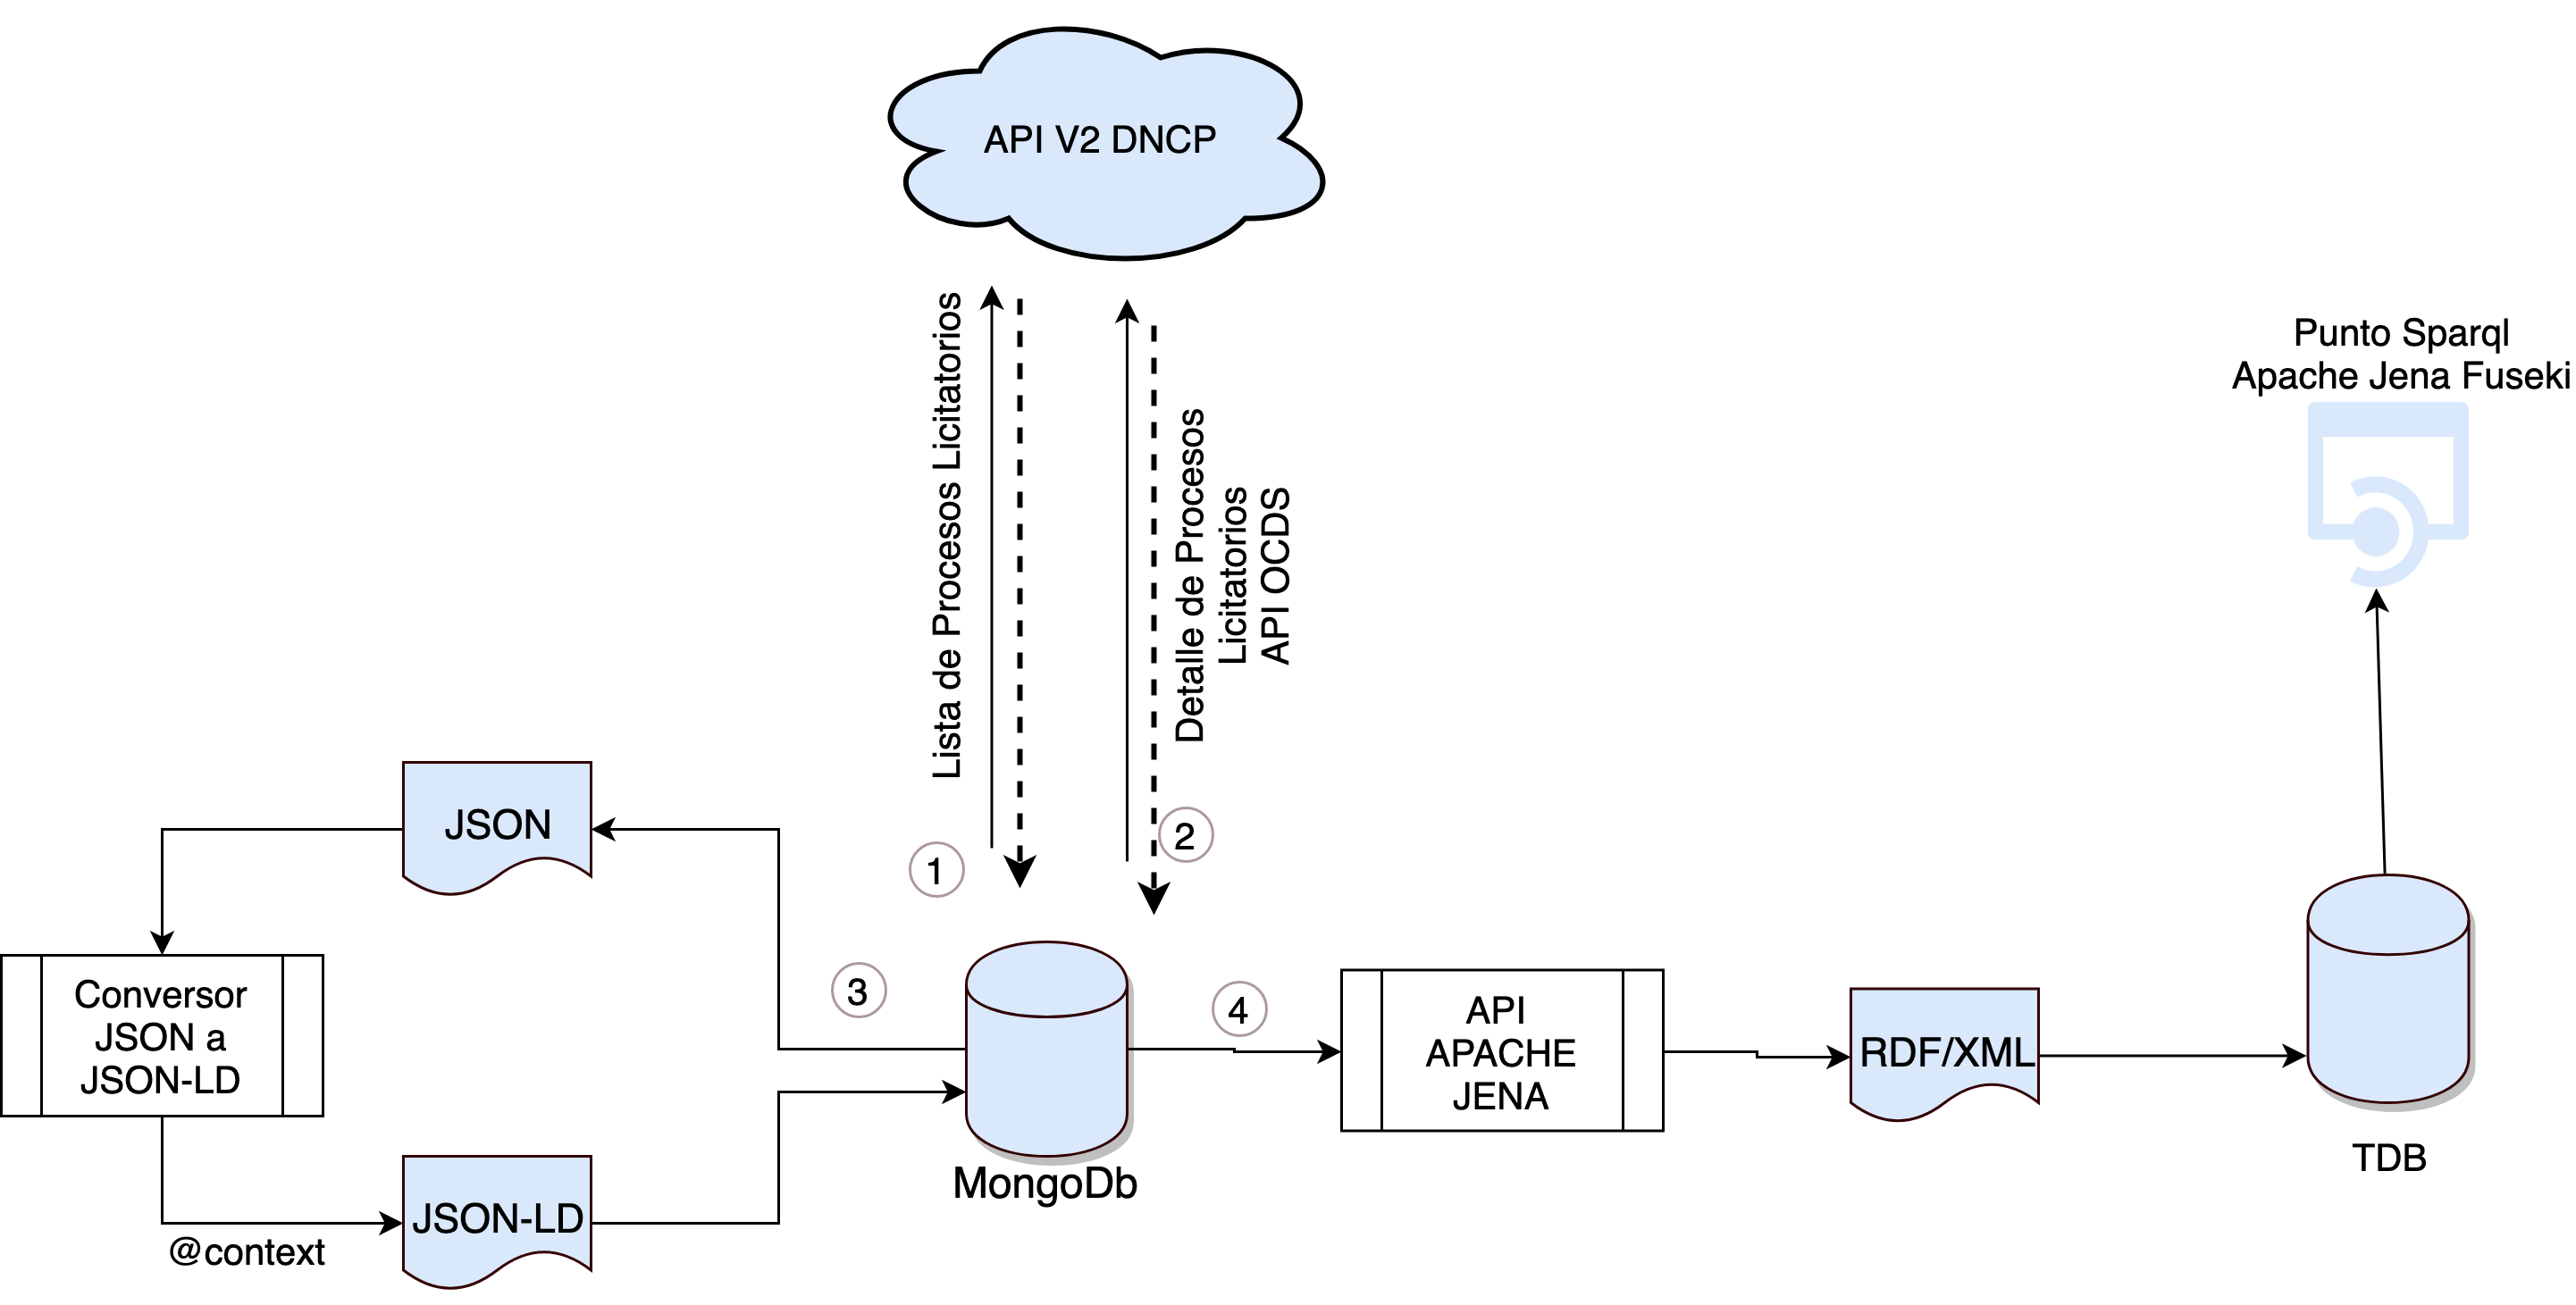
\includegraphics[width=150mm]{figuras/Diagramas-Implementacion.png}
   \caption{Modelo de Implementación}
   \label{img:modelo de Implementacion}
\end{figure}

A continuación explicaremos algunos conceptos relacionados y también las tareas realizadas para lograr montar correctamente el punto SPARQL.


\section{Contexto JSON-LD}

Como se vió anteriormente, existen varias formas de serialización de RDF, en contraste a XML, JSON-LD fue diseñado para ser un formato de intercambio de datos ligero e independiente del lenguaje y es lo suficientemente expresivo como para soportar los conceptos de RDF, además requiere poco esfuerzo para los desarrolladores transformar un documento JSON a JSON-LD\cite{JSONLDJS41:online}. 

Para dar contexto a un objeto JSON es necesario agregar el atributo @context. Éste puede darse de dos formas, definiendo la estructura del contexto como valor de la propiedad, o haciendo referencia (URI) a un documento que contiene la definición del contexto como ya se vió en la sección \ref{section:serializacion_jsonld}.

Se puede ir agregando @context a los objetos hijos de forma recursiva. Esto es muy importante debido a que se pueden sobrescribir los contextos exclusivamente para un objeto en particular sin que afecte a la definición de los demás. Más adelante en este capítulo se abordarán cada uno de los temas.



 




\begin{lstlisting}[captionpos=b, caption=SPARQL query, label=lst:sparql,  numbers=left,  numberstyle=\tiny\color{mygray},
    basicstyle=\ttfamily,frame=single]
 PREFIX java: <http://evolizer.org/ontologies/seon/2009/06/java.owl#>
 PREFIX rdf: <http://www.w3.org/1999/02/22-rdf-syntax-ns#>
 PREFIX rdfs: <http://www.w3.org/2000/01/rdf-schema#>
 SELECT ?url ?name
 WHERE {
    ?url rdf:type java:Package .
    ?url rdfs:label ?name
 }
 \end{lstlisting}

